\section{Background}

\subsection{Analysis of Orientation}

	Analyses of the simulated systems were performed to characterize the orientation of \suldiox in various environments above, within, and below the surface water region. The orientation of the surface molecules as \suldiox adsorbs and interacts with water is a property of any hydrate complex formation that takes places. Better understanding of the molecular orientational distributions will help elucidate the chemistry occurring during the adsorption process.

	The two molecules studied, \wat~and \suldiox, and similarly shaped with a C2$_v$ axis along their bisectors, and a molecular plane is defined by their three atoms. An body-fixed frame is defined for \wat~and \suldiox~as shown in figure \ref{fig:molecular-frame}. In each analysis a world-fixed reference axis is used that is the long axis of the system's periodic cell (normal to the plane of the water surface) unless otherwise noted. The orientational analyses presented herein focus on two angles used to define molecular orientation in space. 
	
	A ``tilt'' angle, $\theta$, defines the angle formed between the bisector vector (the molecular z-axis, pointing from the central atom in the direction of the other two atoms) and the positive system reference axis. Thus the value of $\theta$ falls within a range of $[0,\pi]$. An angle of $\theta=0$ indicates a molecule with its bisector aligned with the reference axis, while $\theta=\pi$ results from an anti-aligned configuration. 
	
	A second angle, $\phi$, defines the molecular ``twist''. $\phi$ is the angle formed between the vector normal to the plane of the molecule (molecular y-axis) and the system reference axis. The values of $\phi$ fall in the interval $[-\pi,\pi]$. Given certain values of $\theta$, $\phi$ provides additional information about whether the molecular orientation is ``flat'' to the surface (e.g. the plane of the molecule is aligned with the plane of the surface), or if it is perpendicular. %However, the symmetry of the \wat~and \suldiox~molecules create equivalence between the two H, or O, atoms (in the \wat~or\suldiox, respectively). $\phi=-\pi$ is equivalent to $\phi=\pi$, and both situations are equivalent to $\phi=0$. Because $\phi=-\phi$, the value is reported within the range of $[0,\frac \pi 2]$. 
	Figure \ref{fig:water-angles} shows the angle definitions relating the body-fixed axes to a system-fixed reference axis. 

%	The two molecules studied, \wat~and \suldiox, and similarly shaped with a C2$_v$ axis along their bisectors, and a molecular plane is defined by their three atoms. The orientational analyses presented herein focus on two angles used to define the molecular orientation in space. In each analysis a reference axis is used to define molecular angles, and is the z-axis unless otherwise specified. A ``tilt'' angle, $\theta$, defines the angle formed between a vector (generally the bisector vector pointing from the central atom in the direction of the other two atoms) and the positive reference axis. Thus the value of $\theta$ falls within a range of $[0,\pi]$. A second angle, $\phi$, defines the molecular ``twist'' around the reference axis. $\phi$ is formed between the projection of a vector onto the x-y reference plane, and the x-axis. $\phi$ is thus defined relative to the x-axis, and its values are in the interval $[-\pi,\pi]$. However, because of the symmetry of the \wat~and \suldiox~molecules and the equivalence of the two H or O atoms (in the \wat~or\suldiox, respectively), $\phi=-\pi$ is equivalent to $\phi=\pi$, and both situations are equivalent to $\phi=0$. Because $\phi=-\phi$, the value is reported within the range of $[0,\frac \pi 2]$. Figure \ref{fig:spherical-angle} shows the angle definitions using the z-axis as the reference axis.

\begin{figure}[h!]
	\begin{center}
		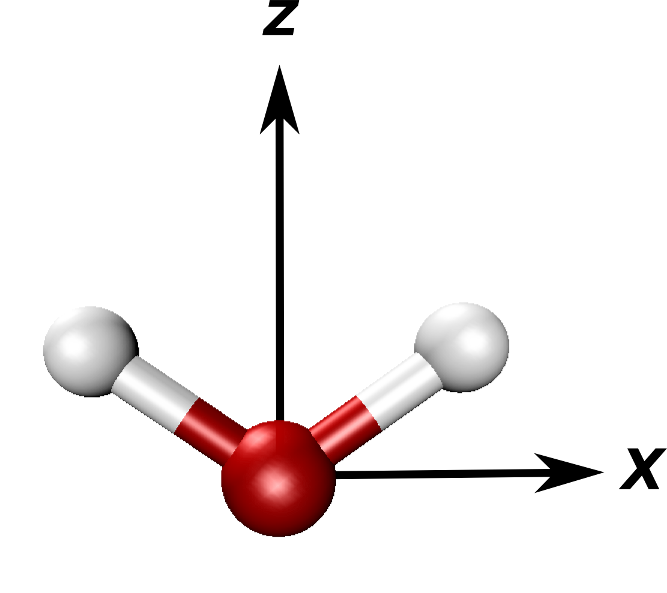
\includegraphics[scale=1.0]{images/molecularframesmall.png}
		\caption{The body-fixed are defined with the molecular plane in the x-z plane, and the z-axis aligned to the molecular bisector. This sets the y-axis normal to the molecular plane, and one of the molecular bonds in the positive x direction.}
		\label{fig:molecular-frame}
	\end{center}
\end{figure}

\begin{figure}[h!]
	\begin{center}
		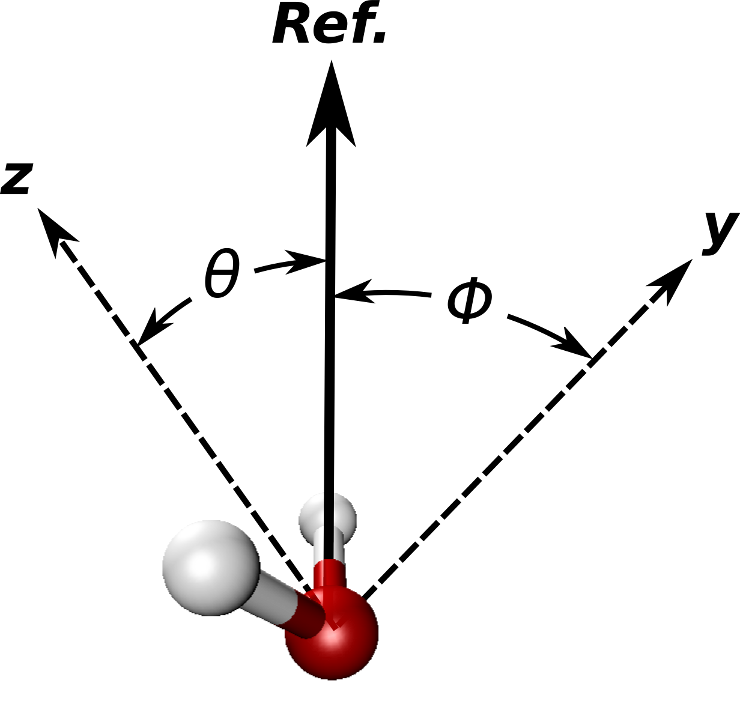
\includegraphics[scale=1.0]{images/wateranglessmall.png}
		\caption{The visual representation of the angles $\theta$ and $\phi$ used to define molecular orientation of \suldiox~and \wat~relative to the reference axis. $\theta$ is the value of the ``tilt'' of the molecular bisector, and $\phi$ is the ``twist'' that indicates how flat the molecule is relative to the interfacial plane.}
		\label{fig:water-angles}
	\end{center}
\end{figure}

\subsubsection{Water Orientation}
The orientation of water molecules at the 

\subsubsection{\suldiox~Orientation}

\subsection{Bonding Analysis}
\subsubsection{Nearest Neighbor}
\subsubsection{Hydrate Complex Formation}
